\documentclass[tikz, border=20pt]{standalone}
\usepackage{tikz}
\usetikzlibrary{shapes.geometric, shapes.symbols, arrows.meta, positioning, fit, backgrounds, calc}

\begin{document}

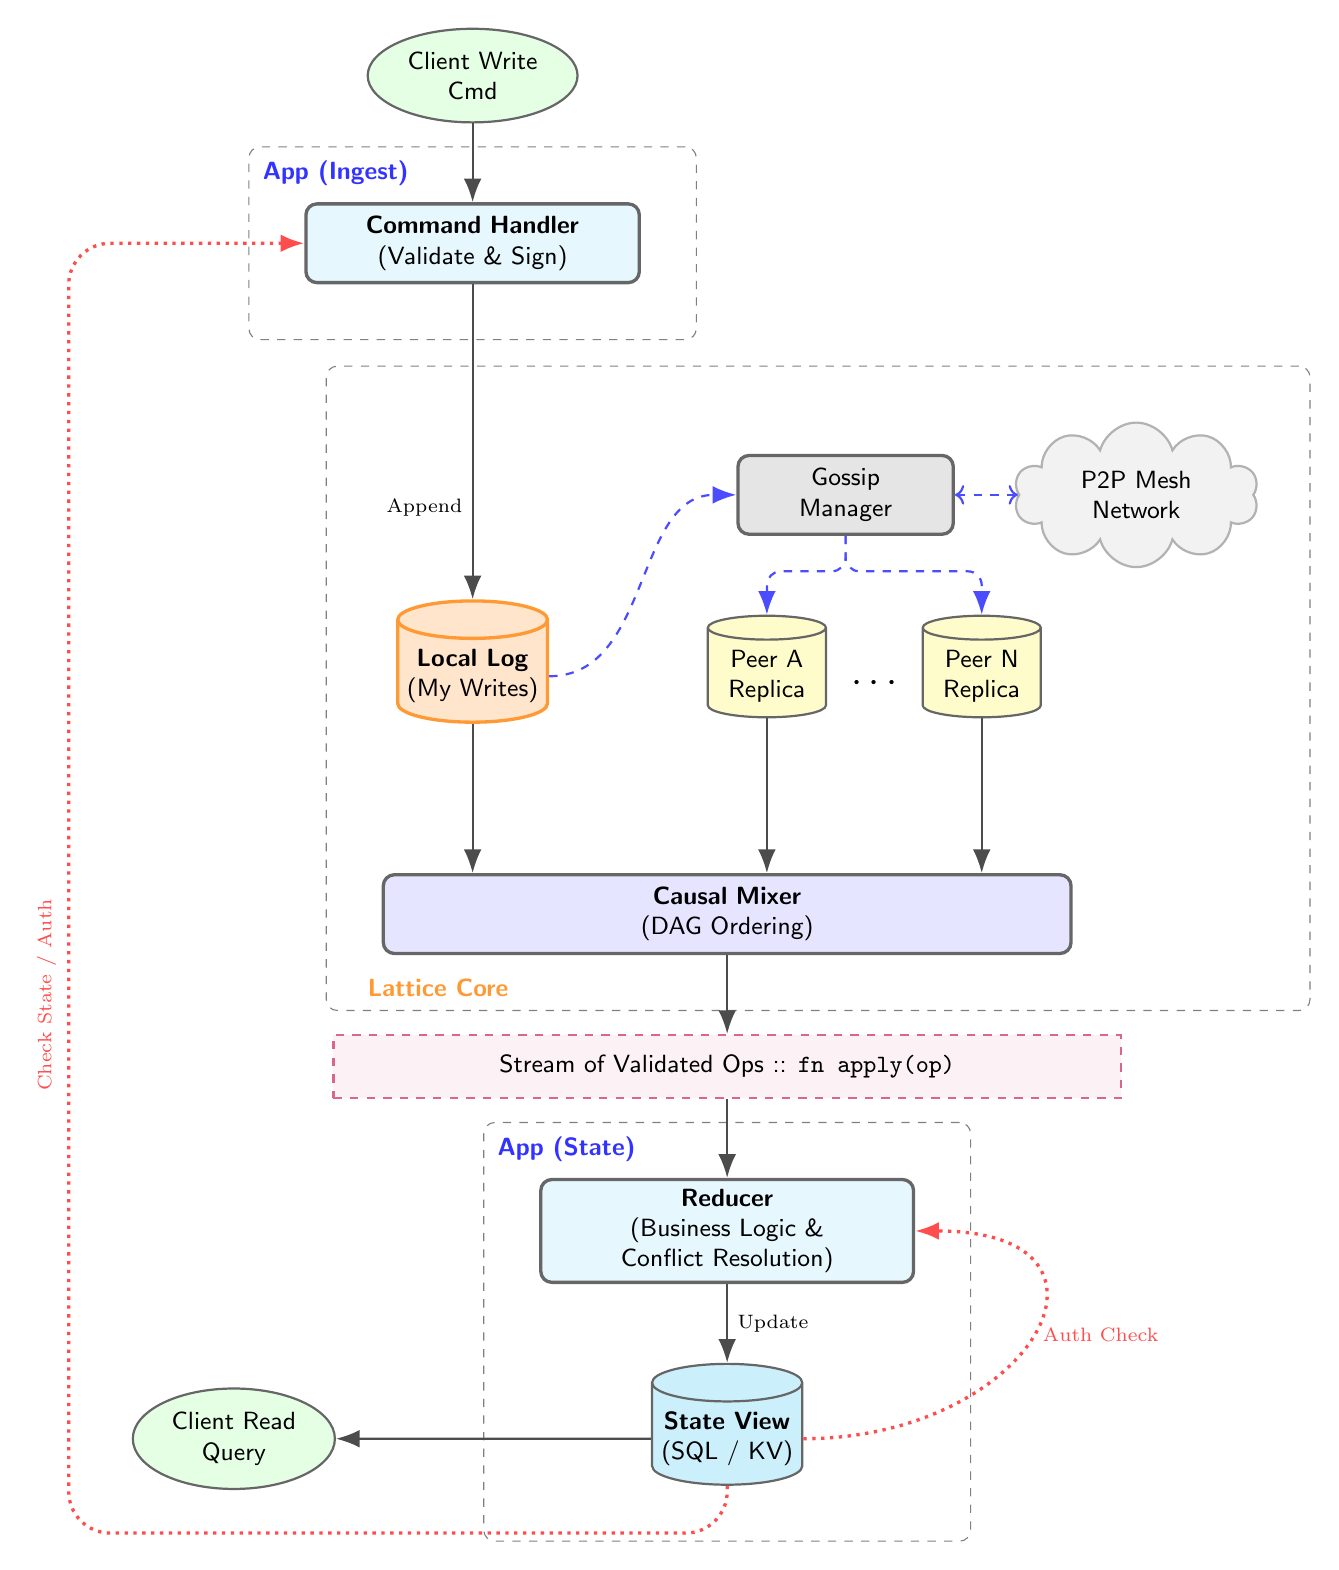
\begin{tikzpicture}[
    node distance=1.5cm and 1.0cm,
    font=\sffamily\small,
    % --- Styles ---
    process/.style={rectangle, draw=black!60, fill=blue!10, very thick, minimum size=1cm, minimum width=2.5cm, rounded corners, align=center},
    storage/.style={cylinder, shape border rotate=90, draw=black!60, fill=yellow!20, thick, aspect=0.25, minimum height=1.2cm, minimum width=1.5cm, align=center},
    highlighted_storage/.style={cylinder, shape border rotate=90, draw=orange!80, fill=orange!20, very thick, aspect=0.25, minimum height=1.2cm, minimum width=1.5cm, align=center},
    interface/.style={rectangle, draw=purple!60, dashed, fill=purple!5, thick, minimum width=10cm, minimum height=0.8cm, align=center},
    cloud_net/.style={cloud, draw=gray!60, fill=gray!10, thick, aspect=2.5, minimum width=3cm, align=center},
    client/.style={ellipse, draw=black!60, fill=green!10, thick, minimum width=2.5cm, align=center},
    group_box/.style={draw=gray, dashed, inner sep=20pt, rounded corners, fill=white, fill opacity=0.0},
    % Line Styles
    arrow/.style={-{Latex[length=3mm]}, thick, draw=black!70, rounded corners=5pt},
    sync_arrow/.style={-{Latex[length=3mm]}, dashed, thick, draw=blue!70, rounded corners=5pt},
    feedback_arrow/.style={-{Latex[length=3mm]}, dotted, very thick, draw=red!70}
]

    % --- Row 1: Client ---
    \node[client] (write_cmd) {Client Write\\Cmd};

    % --- Row 2: Validator (Aligned straight down) ---
    \node[process, below=1cm of write_cmd, fill=cyan!10, text width=4cm] (validator) {\textbf{Command Handler}\\(Validate \& Sign)};

    % --- Row 3: Logs (Storage Layer) ---
    % 1. Local Log
    \node[highlighted_storage, below=4.0cm of validator] (local_log) {\textbf{Local Log}\\(My Writes)};
    
    % 2. Remote Logs
    \node[storage, right=2.0cm of local_log] (remote_log1) {Peer A\\Replica};
    \node[storage, right=1.2cm of remote_log1] (remote_log2) {Peer N\\Replica};
    
    % Dots
    \path (remote_log1) -- node[font=\Large, yshift=-0.1cm] (dots) {$\cdots$} (remote_log2);
    
    % --- Row 2.5: Gossip & Network (Control Plane) ---
    \node[process, above=1.0cm of remote_log1, xshift=1cm, fill=gray!20, text width=2.5cm] (gossip) {Gossip\\Manager};
    
    % Network
    \node[cloud_net, right=0.8cm of gossip] (network) {P2P Mesh\\Network};


    % --- Row 4: Consensus ---
    \coordinate (logs_center) at ($(local_log)!0.5!(remote_log2)$);
    % Removed "& Conflict Resolution" from here as it only handles ordering
    \node[process, below=2.5cm of logs_center, text width=8.5cm] (mixer) {\textbf{Causal Mixer}\\(DAG Ordering)};


    % --- Row 5: Boundary ---
    \node[interface, below=1.0cm of mixer] (boundary) {Stream of Validated Ops :: \texttt{fn apply(op)}};


    % --- Row 6: App Logic ---
    % Added "& Conflict Resolution" here as semantic merging happens in the Reducer
    \node[process, below=1.0cm of boundary, fill=cyan!10, text width=4.5cm] (reducer) {\textbf{Reducer}\\(Business Logic \& Conflict Resolution)};
    
    % --- Row 7: View ---
    \node[storage, below=1.0cm of reducer, fill=cyan!20] (view) {\textbf{State View}\\(SQL / KV)};

    % --- Read Query ---
    \node[client, left=4.0cm of view] (read_query) {Client Read\\Query};


    % --- Background Groups ---
    \begin{pgfonlayer}{background}
        % Core Group
        \node[group_box, fit=(local_log) (network) (mixer) (gossip), fill=yellow!5, label={[anchor=south west, color=orange!80, inner sep=5pt, xshift=10pt]south west:\textbf{Lattice Core}}] (core_group) {};
        
        % App Group TOP (Ingest)
        \node[group_box, fit=(validator), fill=cyan!5, label={[anchor=north west, color=blue!80, inner sep=5pt]north west:\textbf{App (Ingest)}}] (app_group_top) {};

        % App Group BOTTOM (State)
        % Define explicit coordinate for expansion
        \coordinate (app_group_limit) at ($(view.east)+(1.2cm,0)$);
        \node[group_box, fit=(reducer) (view) (app_group_limit), fill=cyan!5, label={[anchor=north west, color=blue!80, inner sep=5pt]north west:\textbf{App (State)}}] (app_group_bottom) {};
    \end{pgfonlayer}


    % --- CONNECTIONS ---

    % 1. Write Path
    \draw[arrow] (write_cmd) -- (validator);
    \draw[arrow] (validator) -- node[left, font=\scriptsize, align=right, pos=0.71] {Append} (local_log);

    % 2. Feedback Loop
    \coordinate (feedback_channel) at ($(read_query.west) + (-0.8cm, 0)$);
    \coordinate (bottom_clearance) at ($(view.south) + (0, -0.6cm)$);
    
    \draw[feedback_arrow, rounded corners=15pt] (view.south) 
        -- (bottom_clearance) 
        -- (bottom_clearance -| feedback_channel) 
        -- node[midway, left, rotate=90, font=\scriptsize, text=red!70, yshift=8pt] {Check State / Auth} (feedback_channel |- validator.west) 
        -- (validator.west);

    % 3. Feed Path
    \draw[arrow] (local_log.south) -- (local_log.south |- mixer.north);
    \draw[arrow] (remote_log1.south) -- (remote_log1.south |- mixer.north);
    \draw[arrow] (remote_log2.south) -- (remote_log2.south |- mixer.north);

    % 4. Sync Path
    % Depart from East instead of North
    \draw[sync_arrow] (local_log.east) to[out=0, in=180] (gossip.west);
    
    % Forked Gossip Arrows
    % Calculate a split point halfway between Gossip and Remote Logs
    \coordinate (sync_split_y) at ($(gossip.south)!0.45!(remote_log1.north)$);
    
    % Draw common trunk then split
    % We draw two paths starting from gossip.south that overlap on the vertical segment
    % This creates the visual of a single line splitting
    \draw[sync_arrow] (gossip.south) -- (gossip.south |- sync_split_y) -| (remote_log1.north);
    \draw[sync_arrow] (gossip.south) -- (gossip.south |- sync_split_y) -| (remote_log2.north);
    
    \draw[sync_arrow, <->] (gossip) -- (network);

    % 5. Execution Path
    \draw[arrow] (mixer) -- (boundary);
    \draw[arrow] (boundary) -- (reducer);
    \draw[arrow] (reducer) -- node[right, font=\scriptsize] {Update} (view);

    % 7. Internal Reducer Check
    \draw[feedback_arrow] (view.east) to[out=0, in=0, looseness=2.5] node[right, font=\scriptsize, text=red!70] {Auth Check} (reducer.east);

    % 6. Read Path
    \draw[arrow] (view) -- (read_query);

\end{tikzpicture}

\end{document}